\subsection{Dataset and preprocessing}

The experiments use Alibaba \texttt{cluster-trace-v2018}. According to the official trace documentation, the release contains approximately 4000 machines over 8 days and provides machine-level utilization, container-level usage, and batch-workload tables \citep{alibabav2018trace}. The study uses three routes from this release: an aggregate series derived from \texttt{machine\_usage}, a high-coverage machine cohort derived from the same archive, and an expanded service-level cohort built by combining \texttt{container\_meta} with a full local mirror of \texttt{container\_usage.tar.gz}.

The preprocessing script reads machine-usage CSV records directly from the tar archive, retains the required columns, drops invalid rows, aggregates the workload by timestamp, and emits a compact CSV at one-minute granularity. The output contains:
\begin{itemize}
  \item mean cluster CPU utilization,
  \item mean cluster memory utilization, and
  \item the number of active machines.
\end{itemize}
This design keeps the aggregate route simple enough to audit directly, while the later machine and service routes progressively narrow the construct-validity gap. The service route now uses a verified local mirror of the full \texttt{container\_usage.tar.gz} archive rather than a streamed prefix subset, which removes the earlier dependence on low-\texttt{container\_id} extraction heuristics.

\subsection{High-coverage machine cohort}

To move beyond a single aggregate time series, the experimental pipeline also extracts a high-coverage machine cohort from the same Alibaba artifact. The cohort builder first scans the raw \texttt{machine\_usage.tar.gz} archive, selects the 12 machines with the highest row counts, aggregates their samples to one-minute means, and then reindexes every entity onto the common global minute span. Missing minutes are marked explicitly and filled by interpolation only after selection. The retained machines cover between 93.7\% and 94.7\% of the global minute span, with an average imputation ratio of 5.8\%.

This second dataset is not presented as a full service-level benchmark. Its purpose is narrower and more practical: to test whether the forecasting conclusions observed on the aggregate series collapse immediately when the unit of analysis changes from one cluster-wide series to multiple long-lived machine-level series.

\subsection{Container service cohort}

To narrow the remaining construct-validity gap, the pipeline also extracts an expanded service-level cohort from the official Alibaba container tables. The route starts from \texttt{container\_meta.tar.gz}, which exposes container-to-\texttt{app\_du} membership and per-container request sizes. A full pass over the mirrored \texttt{container\_usage.tar.gz} archive then drops rows with blank container identifiers, maps each retained row back to its parent \texttt{app\_du}, and aggregates service demand to one-minute resolution using both mean utilization and a CPU-core proxy computed from the product of requested cores and observed CPU utilization.

The service route now follows a simpler fixed rule. It first applies a metadata prefilter requiring at least 60 containers and at least 650{,}000 seconds of observed span in \texttt{container\_meta}. It then performs a full usage-profile sweep and retains every \texttt{app\_du} group whose matched-container hit ratio is at least 0.90. After service-minute aggregation and reindexing onto the common global span, the final cohort keeps every profiled candidate whose observed-minute coverage remains at least 0.96 and whose matched-container hit ratio remains at least 0.90. Under this rule, the verified broad service cohort contains 139 \texttt{app\_du} groups, 19{,}419 selected containers, and 19{,}269 matched containers over a common 11{,}520-minute span, with an average observed-minute coverage ratio of 97.27\%, a coverage range of 97.23\%--97.30\%, an average matched-container hit ratio of 99.32\%, and an average imputation ratio of 2.73\%. A dedicated top-10 overlap audit retains all 10 services from the earlier targeted cohort. This is therefore a much broader official-data extension, although it still should not be read as a full population census because the metadata prefilter intentionally excludes smaller and shorter-lived services.

\begin{table}[htbp]
  \centering
  \caption{Summary statistics of the broad Alibaba service-level cohort extracted from the official container tables.}
  \label{tab:service-cohort-stats}
  \small
  \begin{tabular}{lc}
    \toprule
    Item & Value \\
    \midrule
    Services (\texttt{app\_du}) & 139 \\
    Selected containers & 19{,}419 \\
    Matched containers in usage stream & 19{,}269 \\
    Common minute span & 11{,}520 \\
    Mean observed-minute coverage & 0.973 \\
    Coverage range & 0.972--0.973 \\
    Mean container hit ratio & 0.993 \\
    Mean imputation ratio & 0.027 \\
    \bottomrule
  \end{tabular}
\end{table}

\begin{table}[htbp]
  \centering
  \caption{Statistics of the processed aggregate Alibaba \texttt{v2018} workload series.}
  \label{tab:dataset-stats}
  \begin{tabular}{lc}
    \toprule
    Item & Value \\
    \midrule
    Observed one-minute samples & 11{,}208 \\
    Minute-index span & 0--11{,}519 \\
    Mean CPU utilization & 37.996\% \\
    Peak CPU utilization & 78.788\% \\
    Mean memory utilization & 88.007\% \\
    Median active machine count & 3994.917 \\
    \bottomrule
  \end{tabular}
\end{table}

\begin{figure}[htbp]
  \centering
  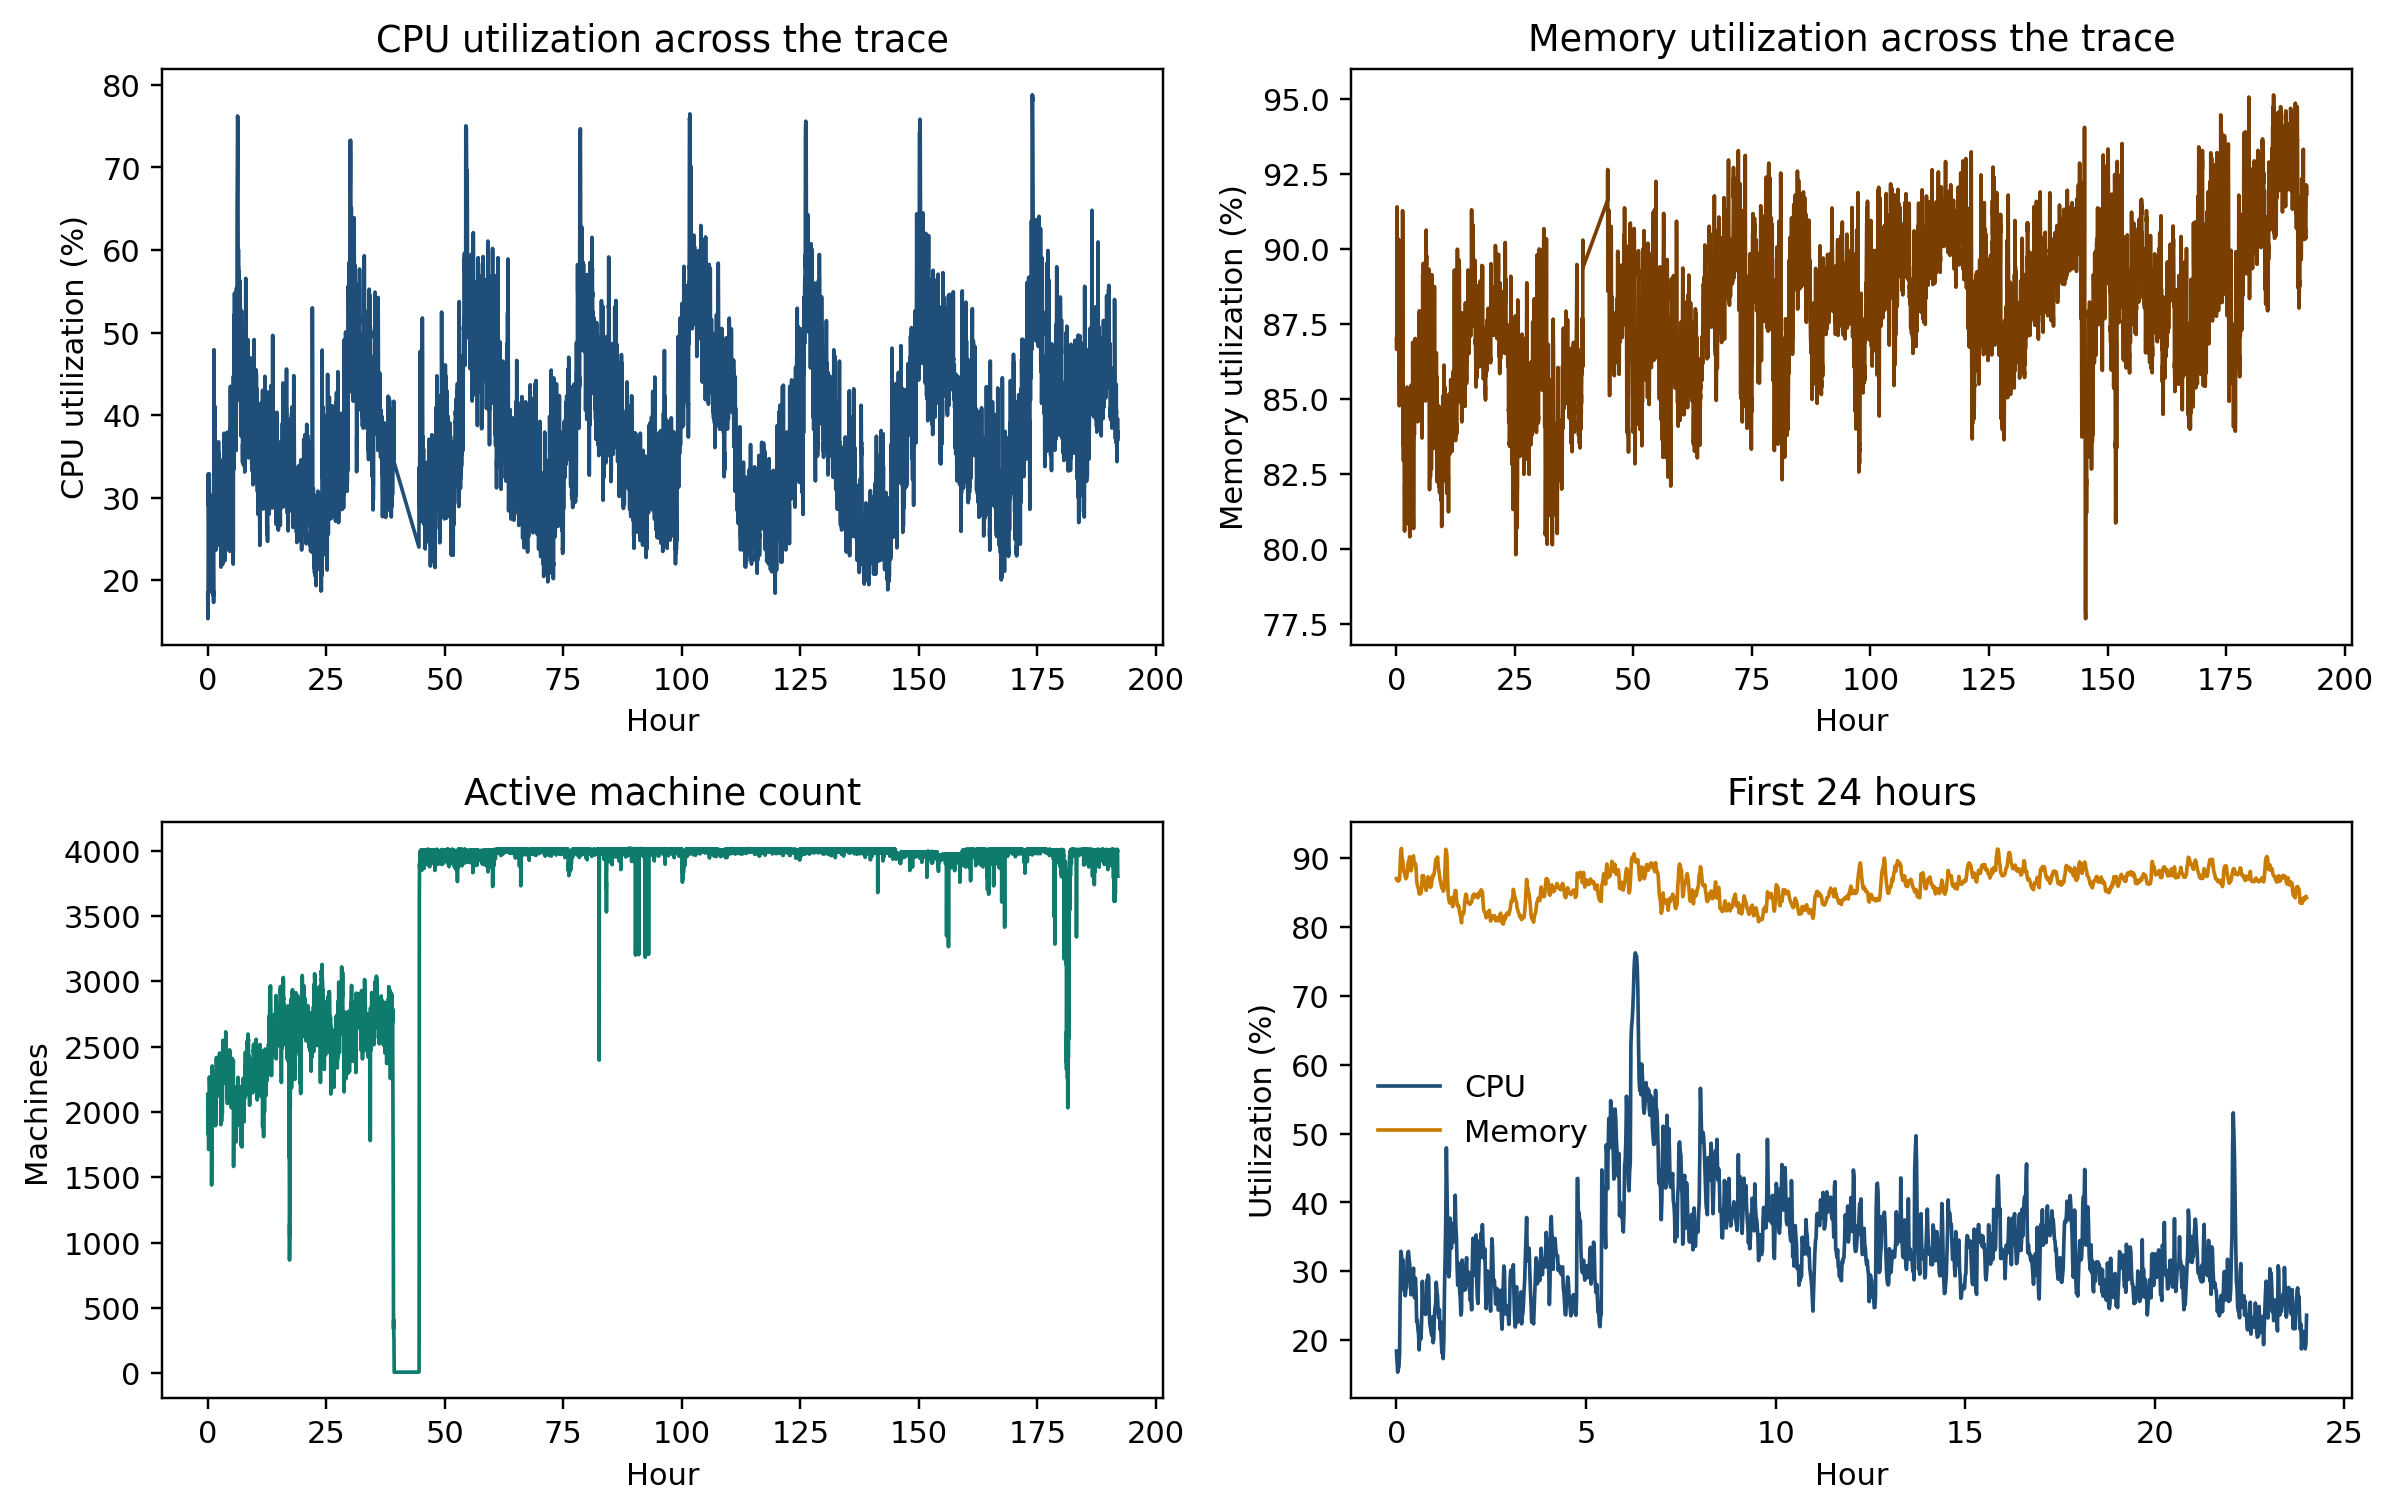
\includegraphics[width=\linewidth]{../experiments/results/figures/cluster_workload_overview.png}
  \caption{Aggregate workload overview across the processed Alibaba \texttt{v2018} series, including CPU, memory, active-machine counts, and the first-day zoom.}
  \label{fig:workload-overview}
\end{figure}

\begin{figure}[htbp]
  \centering
  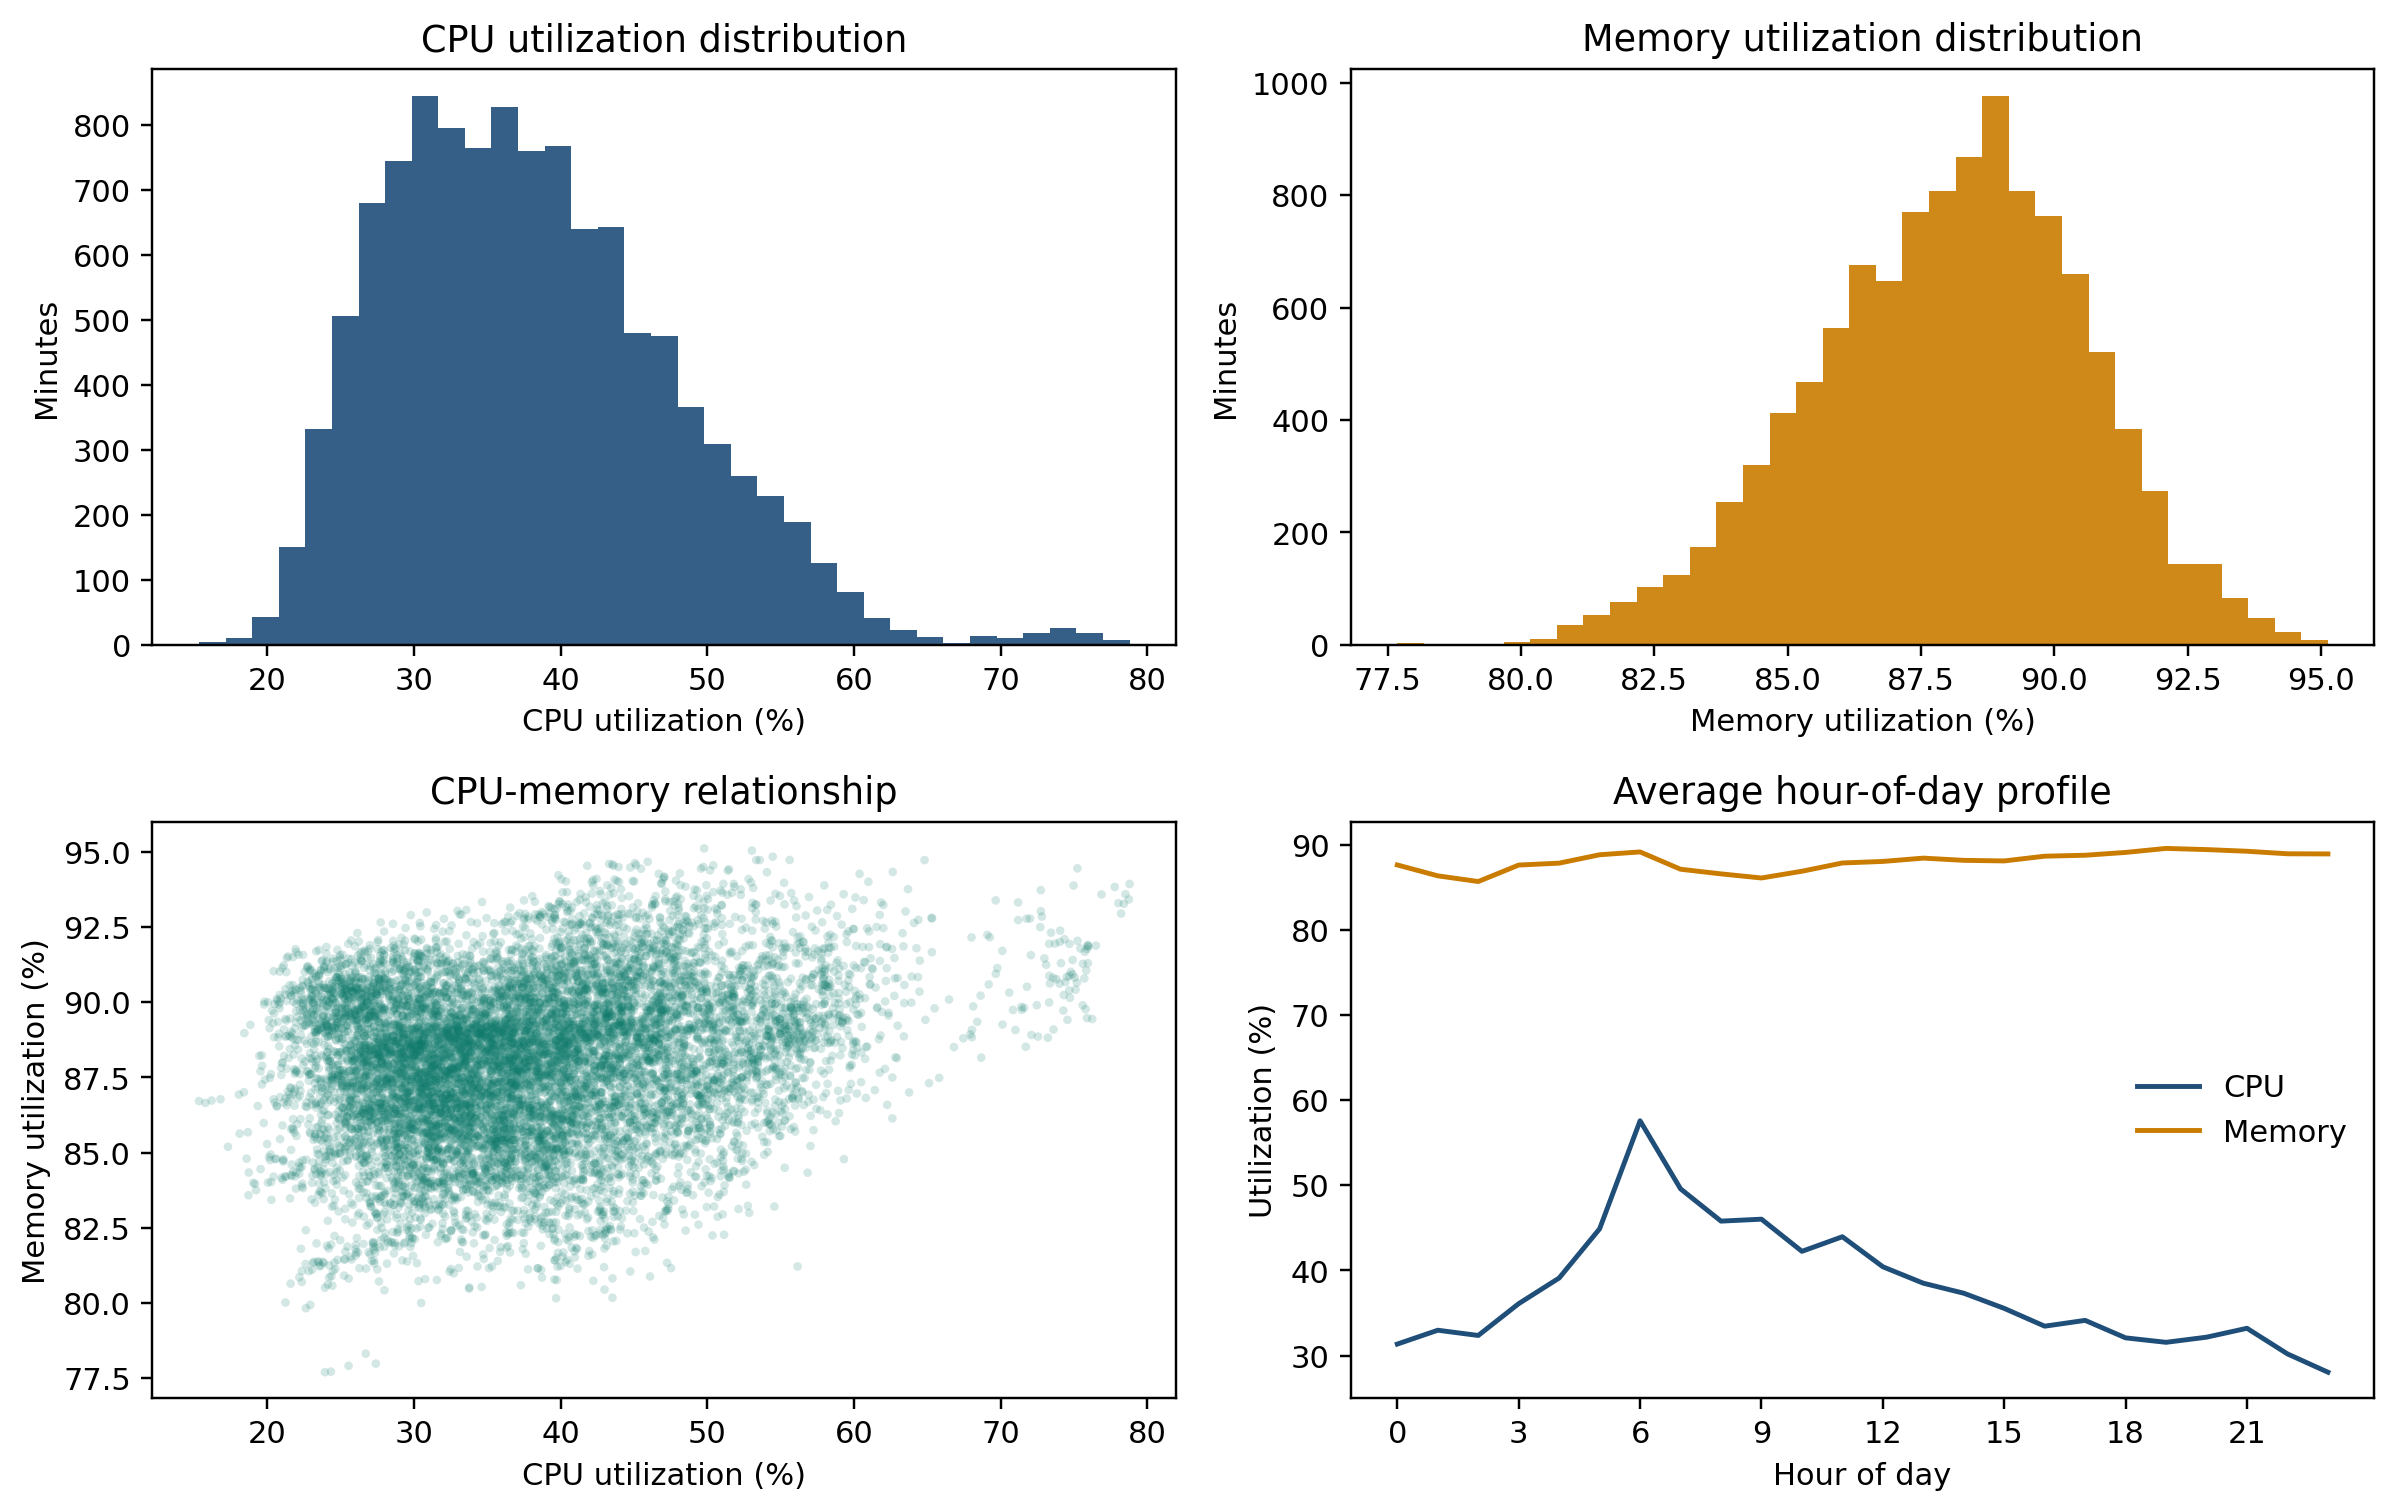
\includegraphics[width=\linewidth]{../experiments/results/figures/resource_distribution_views.png}
  \caption{Additional views of the processed series: CPU distribution, memory distribution, CPU-memory relationship, and average hour-of-day profile.}
  \label{fig:distribution-views}
\end{figure}

\begin{figure}[htbp]
  \centering
  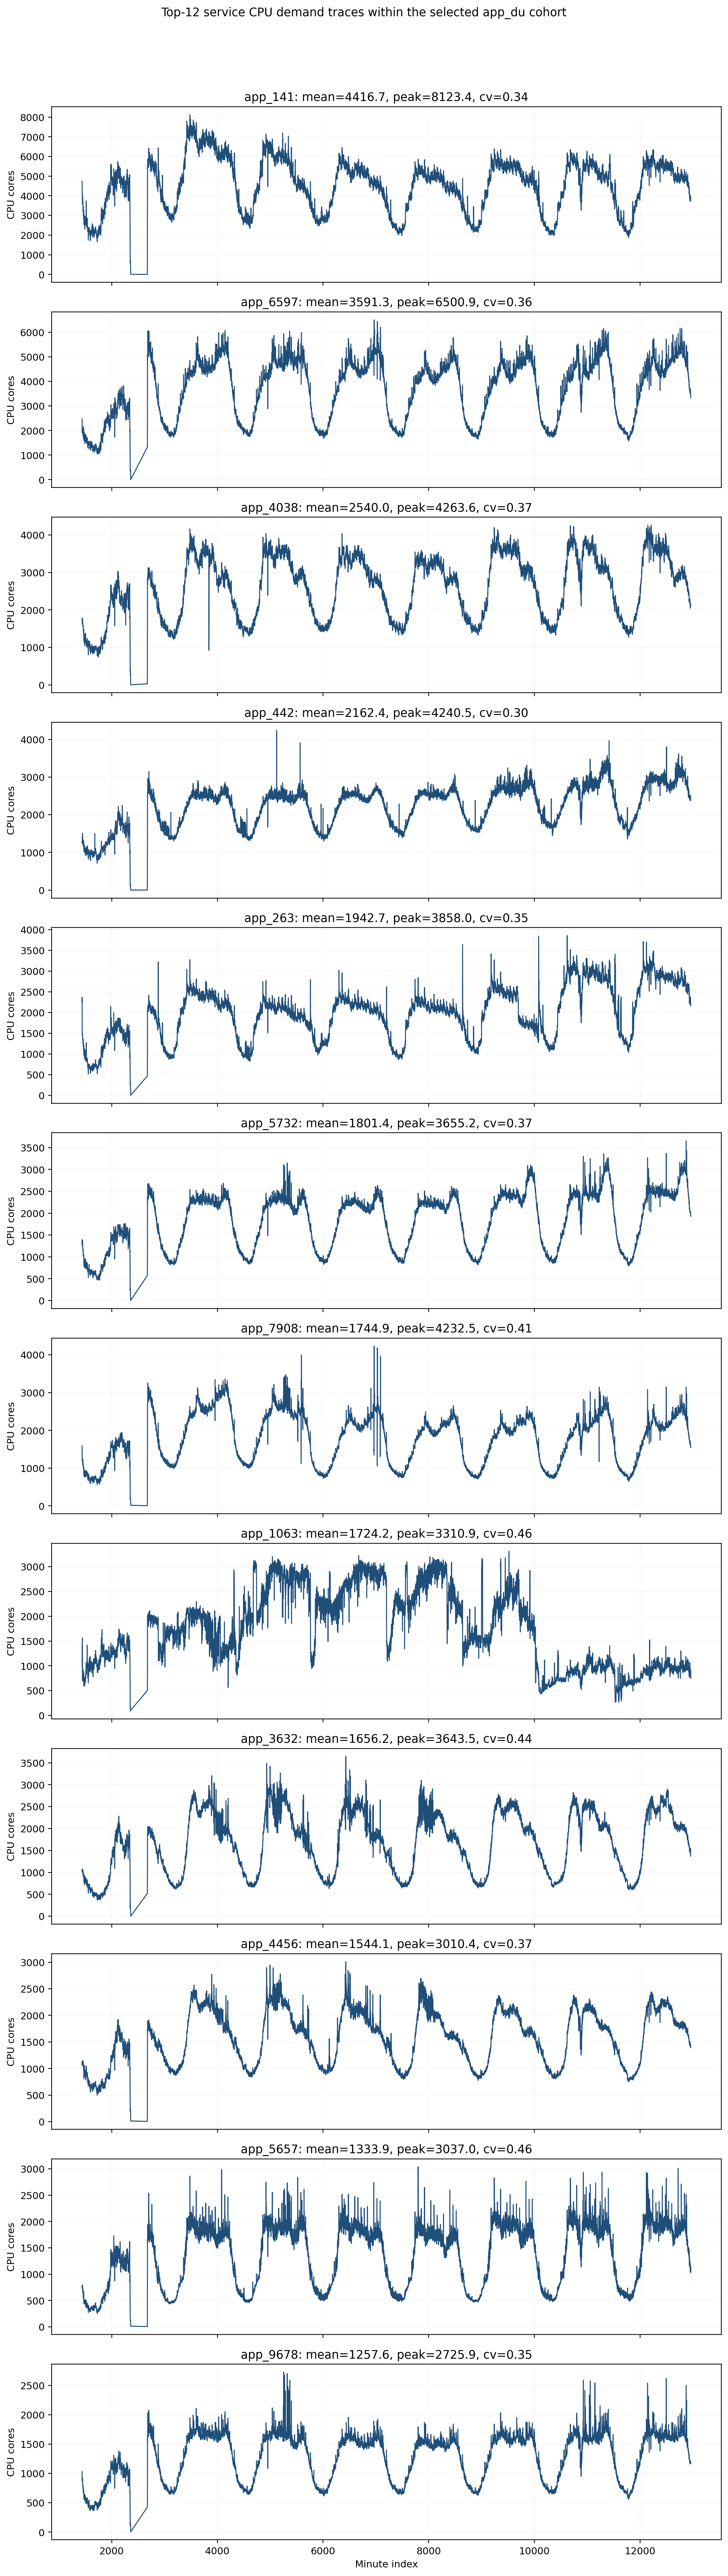
\includegraphics[width=0.78\linewidth]{../experiments/results/service_cohort_broad/figures/service_workload_overview.png}
  \caption{Twelve representative high-demand services from the broad \texttt{app\_du} cohort. Even under the same shared minute span, the retained services differ markedly in mean load, smoothness, and burstiness.}
  \label{fig:service-workload-overview}
\end{figure}

\subsection{Forecasting and policy configuration}

The forecasting benchmark currently implements five point-forecast baselines: persistence, moving average, linear regression, random forest, and a standard feed-forward multilayer perceptron (MLP) regressor. In addition, it implements \texttt{UA-MSTCN-Lite}, a trainable uncertainty-aware surrogate that uses multi-scale history features together with a quantile-aware tree ensemble. The MLP is included as a conventional neural baseline that does not assume a specialized temporal architecture. These models serve two roles. First, they validate the experiment harness without requiring a heavyweight sequence-model stack. Second, they define increasingly strong performance floors that a later deep TCN variant must exceed.

The aggregate series is split chronologically into training, validation, and test segments using a $70/15/15$ partition. The training route consumes the first 85\% of the series, and the test route consumes the final 15\% only; all forecasting numbers reported in this revision use this leakage-free split. The context window is fixed to 60 minutes in the default configuration, and forecast horizons are set to 1, 5, and 10 minutes. This choice balances operational relevance with manageable control lag. Forecasting quality is measured with MAE, RMSE, MAPE, and pinball loss.

The autoscaling simulator compares three policies:
\begin{enumerate}
  \item a reactive threshold policy with upper and lower utilization thresholds, and
  \item a lagged target-tracking policy that follows the previous-step required capacity under the same step-size constraint, and
  \item a predictive policy that uses median and high-quantile forecasts with cooldown and maximum-step constraints.
\end{enumerate}
All three policies act on a normalized aggregate capacity signal. The predictive route uses the calibrated high-quantile forecast for scale-out, adds the configured scale-out margin, and evaluates decisions in the same required-capacity space as the reactive and lagged baselines.

\subsection{Extended analysis protocol}

Beyond the core benchmark tables, the protocol includes six additional analyses:
\begin{enumerate}
  \item \textbf{Context sensitivity:} the \texttt{UA-MSTCN-Lite} context window is varied over 30, 60, and 120 minutes to test short- versus long-history dependence.
  \item \textbf{Regime analysis:} the 5-minute horizon test windows are partitioned into stable, moderate, and bursty subsets according to the local standard deviation of the recent 30-minute history.
  \item \textbf{Quantile calibration:} empirical $P50$ and $P90$ coverage, together with interval width, are measured for the uncertainty-aware surrogate.
  \item \textbf{Policy ablation and sensitivity:} the predictive controller is re-evaluated after removing the scale-out margin, removing cooldown, collapsing to median-only forecasts, and sweeping the scale-out margin/cooldown pair.
  \item \textbf{Cross-machine transfer:} pooled global models are trained on 8 machines and evaluated zero-shot on 4 held-out machines, repeated over 3 deterministic folds.
  \item \textbf{Service-level evidence:} a rule-based broad \texttt{app\_du} cohort extracted from official container tables is used to test both forecast calibration and predictive control at a more natural autoscaling unit.
\end{enumerate}
For the service-level policy route, the protocol fixes the resampling unit to \texttt{service}. The primary comparison statistic is the equal-weighted mean predictive-minus-reactive delta across retained services, while a load-weighted mean delta using the service CPU-cores proxy is reported only as an auxiliary sensitivity check. Stability is assessed with paired bootstrap over services using a fixed resample count and the following interpretation rule for lower-is-better metrics: a 95\% interval fully below zero indicates stable improvement, a 95\% interval fully above zero indicates stable degradation, and an interval that crosses zero is treated as not stable. The same pre-fixed rule also governs service-cohort promotion: a broader audited cohort replaces the earlier targeted mainline if the forecasting headline flips, if a policy headline mean direction flips, or if an earlier declarative gain on service-level over-provisioning or scaling actions is no longer stably supportable.
For the machine cohort, the same leakage-free forecasting setup is reused so that aggregate and cross-entity results remain directly comparable.

\subsection{Artifacts and environment}

The experimental pipeline writes its outputs to \texttt{paper-workbench/experiments/results/}. The metrics contract is fixed by \texttt{metrics.csv}, the policy time series is exported as \texttt{policy\_series.csv}, and the manuscript figures are rendered from these artifacts rather than edited manually. This contract is important because the manuscript should consume experiment outputs directly rather than rely on hand-copied numbers.

The experiments were executed with TeX Live 2023, \texttt{pdflatex}, and \texttt{latexmk} for manuscript compilation, together with a dedicated Python environment containing \texttt{pandas}, \texttt{scikit-learn}, \texttt{pyyaml}, and \texttt{matplotlib}. This keeps the current implementation lightweight and reproducible.
